\documentclass[a4wide]{report}

\usepackage{amsmath}
\usepackage[a4paper, total={7in, 10.2in}]{geometry}
\usepackage{graphicx}
\usepackage[portuguese]{babel}
\usepackage[utf8]{inputenc}


\begin{document}

\noindent
{\bf Rafael V. Cacilhas  - Relatório 04 (\today)}

\vspace{0.5cm}

\section*{Exercício 1}

\subsection*{a) }

Na Figura \ref{1} temos o fator de estrutura pedido.

\begin{figure}[!htb]
\centering
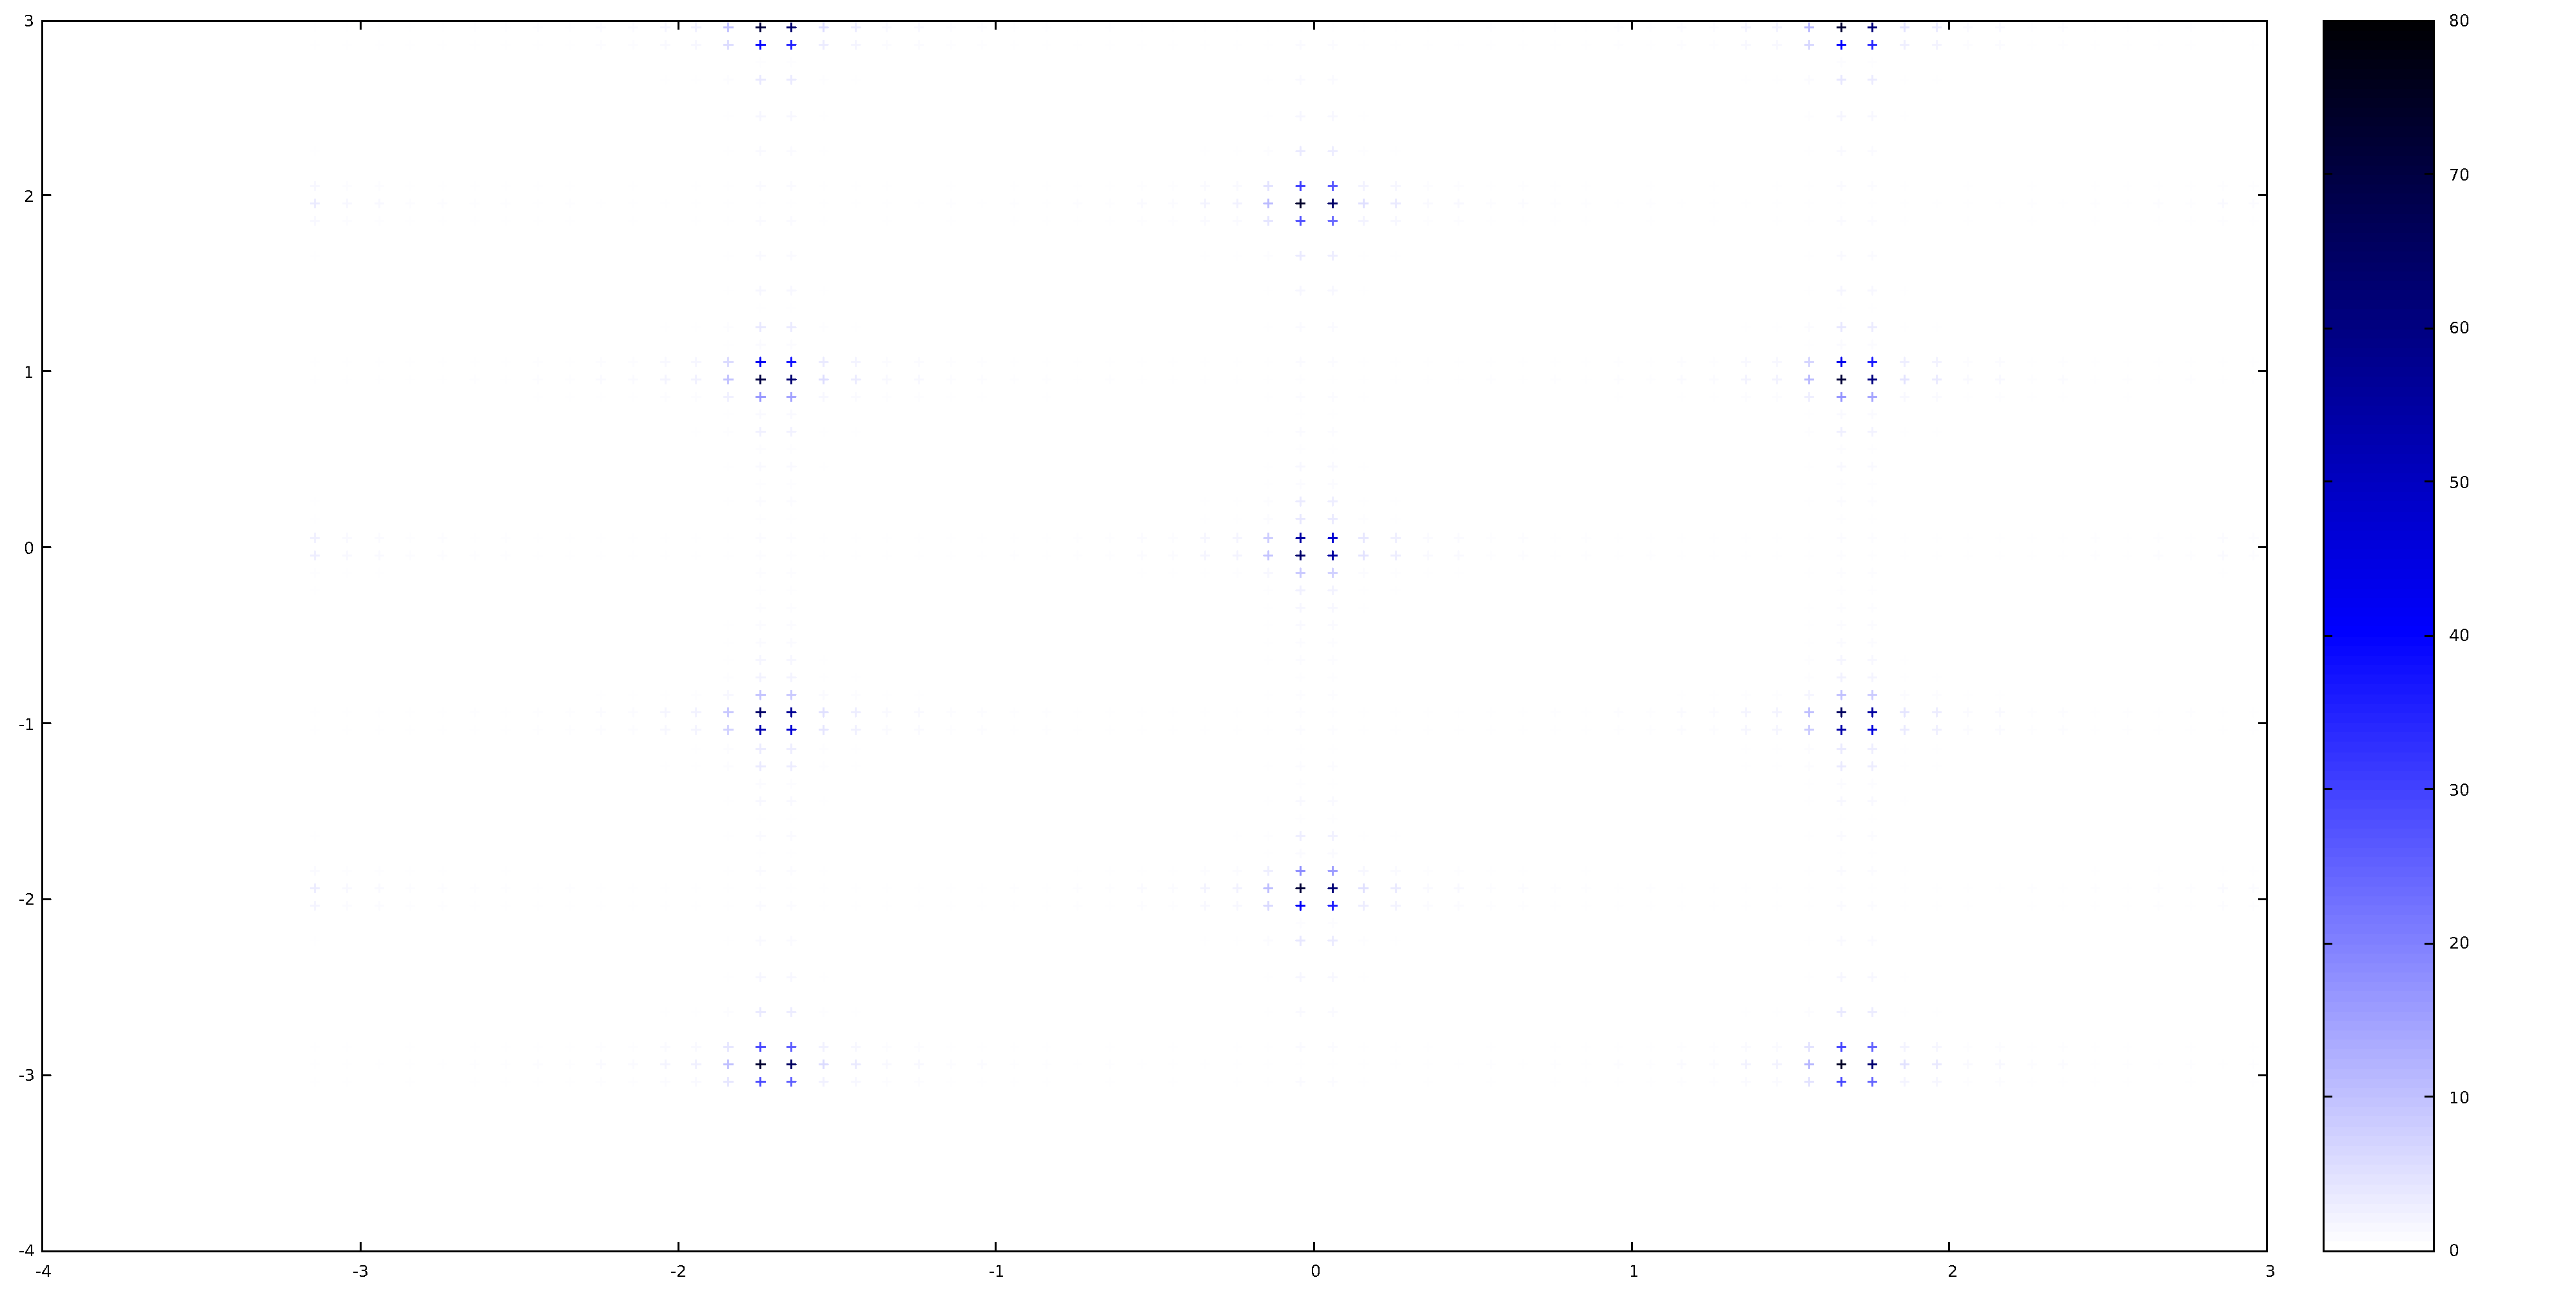
\includegraphics[width=0.447\textwidth]{1.pdf}
\caption{Fator de estrutura.}
\label{1}
\end{figure}



\section*{Exercício 2}

\subsection*{a)}

Os coeficientes $a_n$ e $b_n$ para a função $f(t) = $
$\begin{cases} 
-7, t < t* \\ 
+7, t > t*
\end{cases} $
são: 
\begin{equation}
a_0 = \int_{-T/2}^{T/2} f(t) dt = 0
\end{equation}

\begin{equation}
a_n = \int_{-T/2}^{T/2} f(t) \cos(t) dt = \int_{-T/2}^{0} f(t) \cos(t) dt + \int_{0}^{T/2} f(t) \cos(t) = 0
\end{equation}

\begin{equation*}
b_n = \int_{-T/2}^{T/2} f(t) \sin(t) dt = \int_{-T/2}^{0} f(t) \sin(t) dt + \int_{0}^{T/2} f(t) \sin(t) = 2\int_{0}^{T/2} f(t) \sin(t)
\end{equation*}

\begin{equation}
b_n = \frac{-28}{T \omega_n} \cos(\omega_n t) \bigg|_{0}^{T/2} = -\frac{14}{\pi n} \left[ \cos(n\pi) - 1 \right]
\end{equation}

Ou 
$\begin{cases} 
b_2n = 0 \\ 
b_{2n-1} = \frac{28}{(2n-1) \pi}
\end{cases} $

\vspace{3pt}
Na Figura \ref{a} está o gráfico da função $f(t)$ e as funções $f_{M}(t)$ para diversos M. Como esperado, quanto maior o M mais a função $f_{M}(t)$ se aproxima d $f(t)$ original. A comparação entre M = 3 (vermelho) e M = 55 (marrom) demonstra claramente como a adição de mais termos faz com que a aproximação seja muito melhor.
\begin{figure}[!htb]
\centering
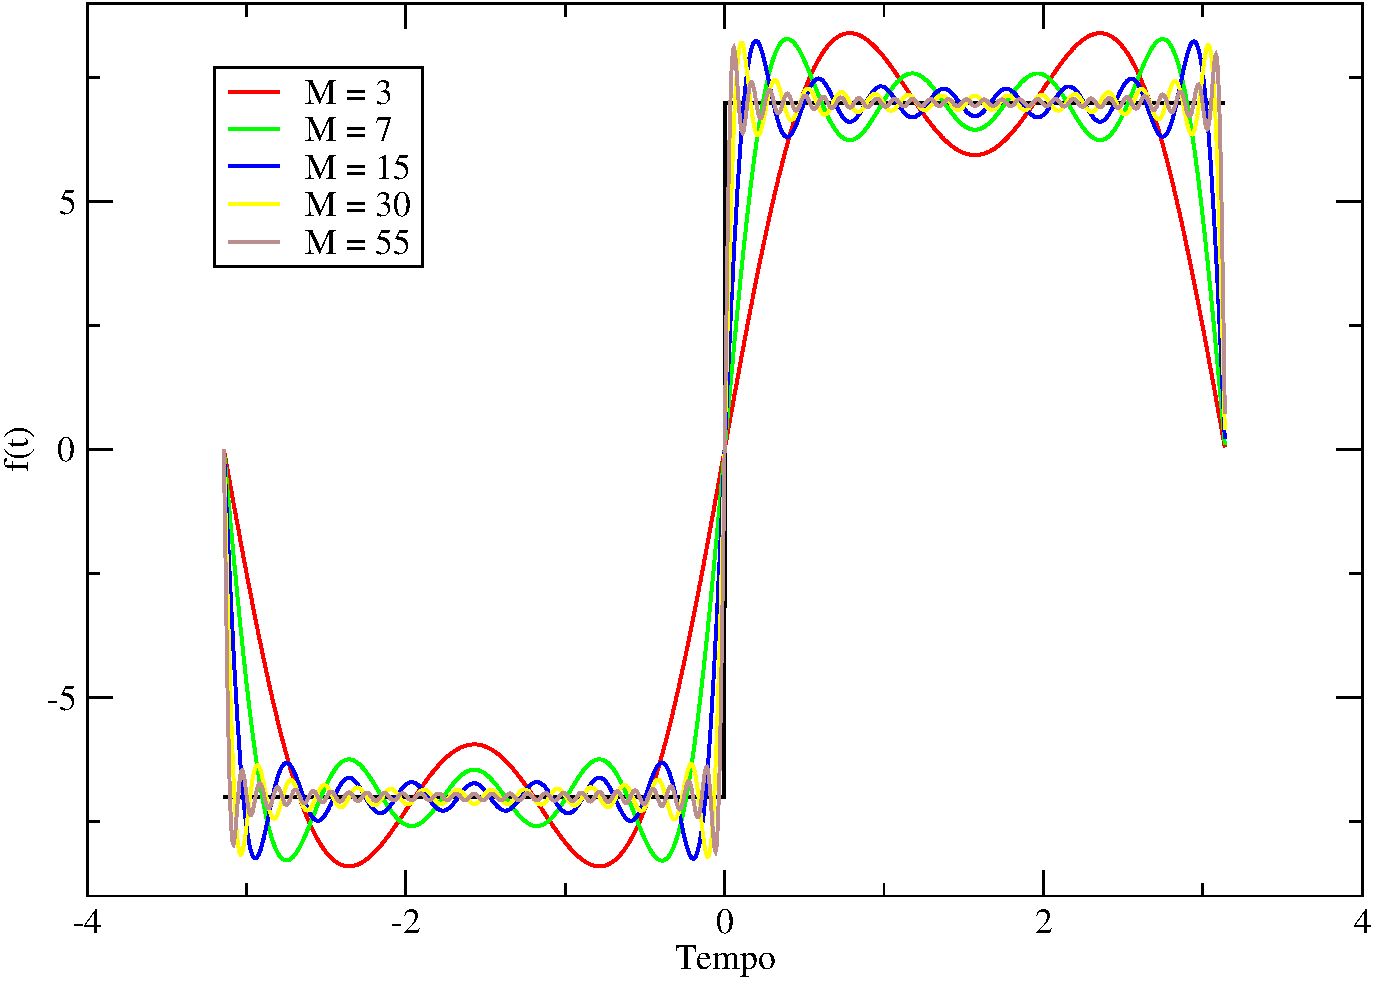
\includegraphics[width=0.447\textwidth]{a.pdf}
\caption{Funções $f_M(t)$ para vários M.}
\label{a}
\end{figure}


\subsection*{b)}

Na Figura \ref{55} foi plotado a função $f_{55}(t)$ para $-4T < t < 4T$. Como esperado, a função $f_{55}(t)$ é periódica, tendo período $ T = 2\pi$
\begin{figure}[!htb]
\centering
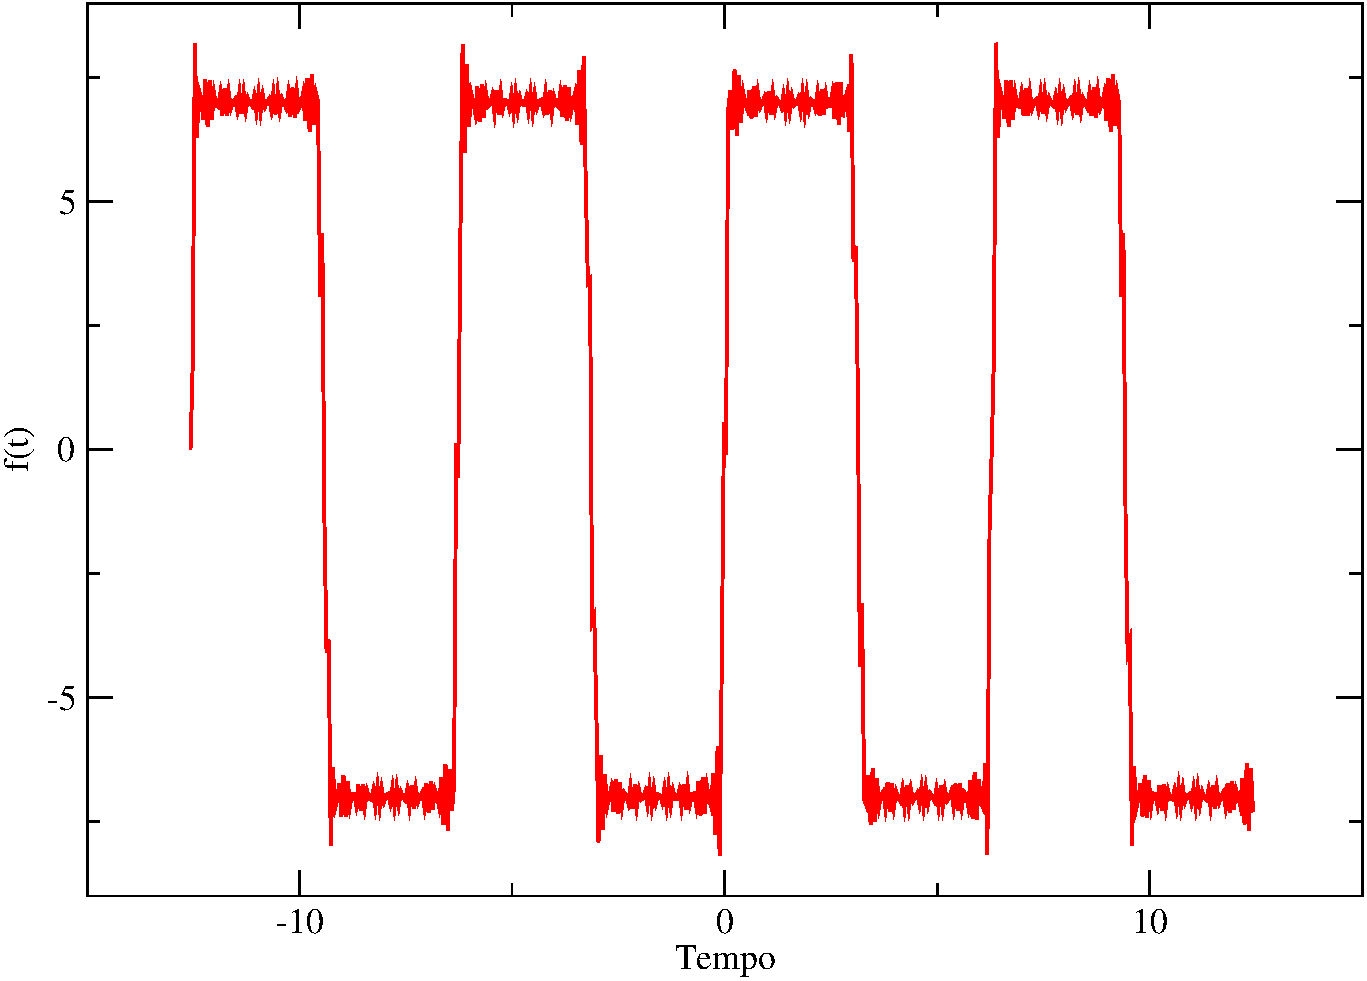
\includegraphics[width=0.447\textwidth]{55.pdf}
\caption{Função $f_{55}(t)$ no intervalo -4T < t < 4T.}
\label{55}
\end{figure}


\subsection*{c)}

Na Figura \ref{c} temos a função $f(t)$ e as funções $f_{M}(t)$ para os parâmetros B = 2 e t* = $\pi / 2$.

\begin{figure}[!htb]
\centering
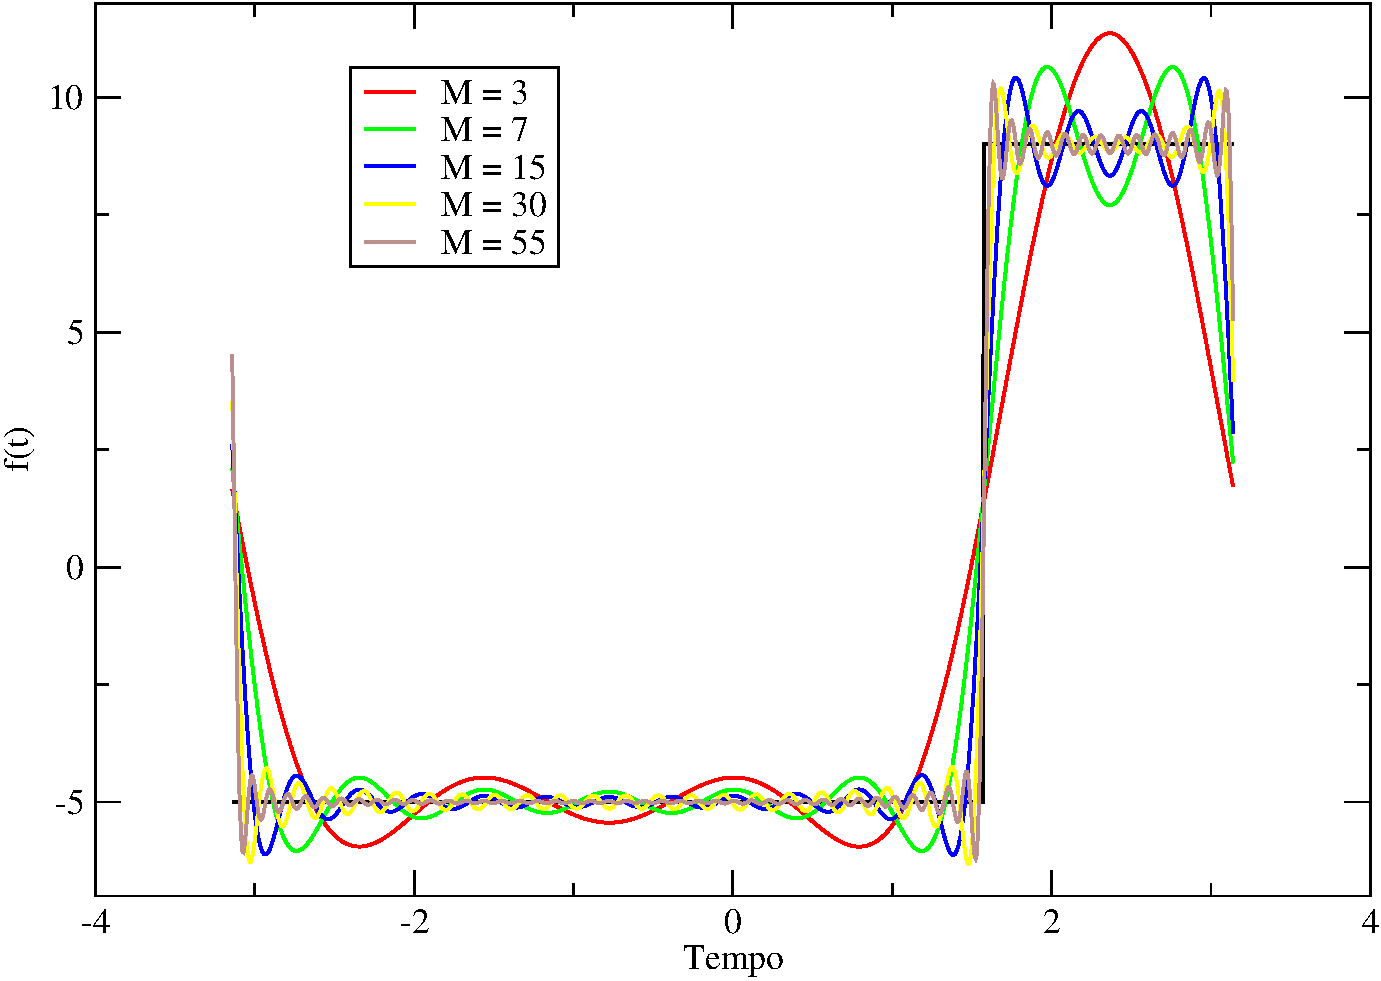
\includegraphics[width=0.447\textwidth]{c.pdf}
\caption{ Funções $f_{M}(t)$  para diversos M com os parâmetros B = 2 e t* = $\pi / 2$.}
\label{c}
\end{figure}


\section*{Exercício 3}
\subsection*{a)}

Na Figura \ref{pot} podemos ver a comparação do espectro de potência entre as séries 1 e 2 e entre as séries 3 e 4. As séries 1 e 2 possuem espectros de potência completamente diferentes, apesar da onda resultante ser muito parecida. A série 1 possui contribuições de várias frequências, ao passo que a série 2 possui contribuições somente de poucas frequências. Já as séries 3 e 4 possuem espectros muito semelhantes, apesar da série 3 possuir alguns picos perto de N = 20 que a série 4 não possui.


\begin{figure}[!htb]
\centering
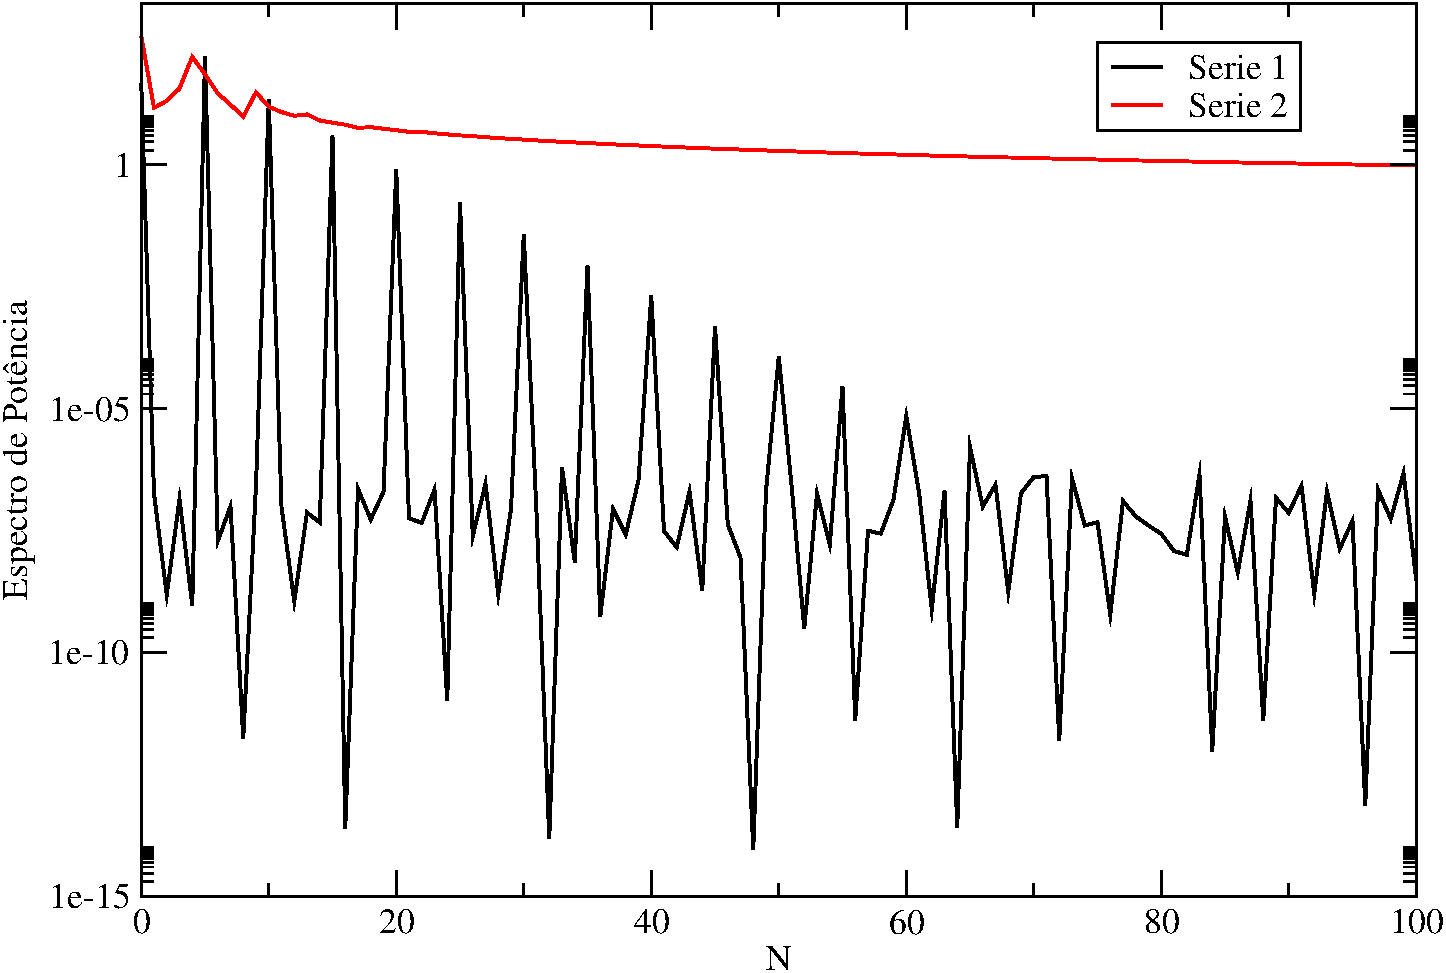
\includegraphics[width=0.447\textwidth]{saida2.pdf}
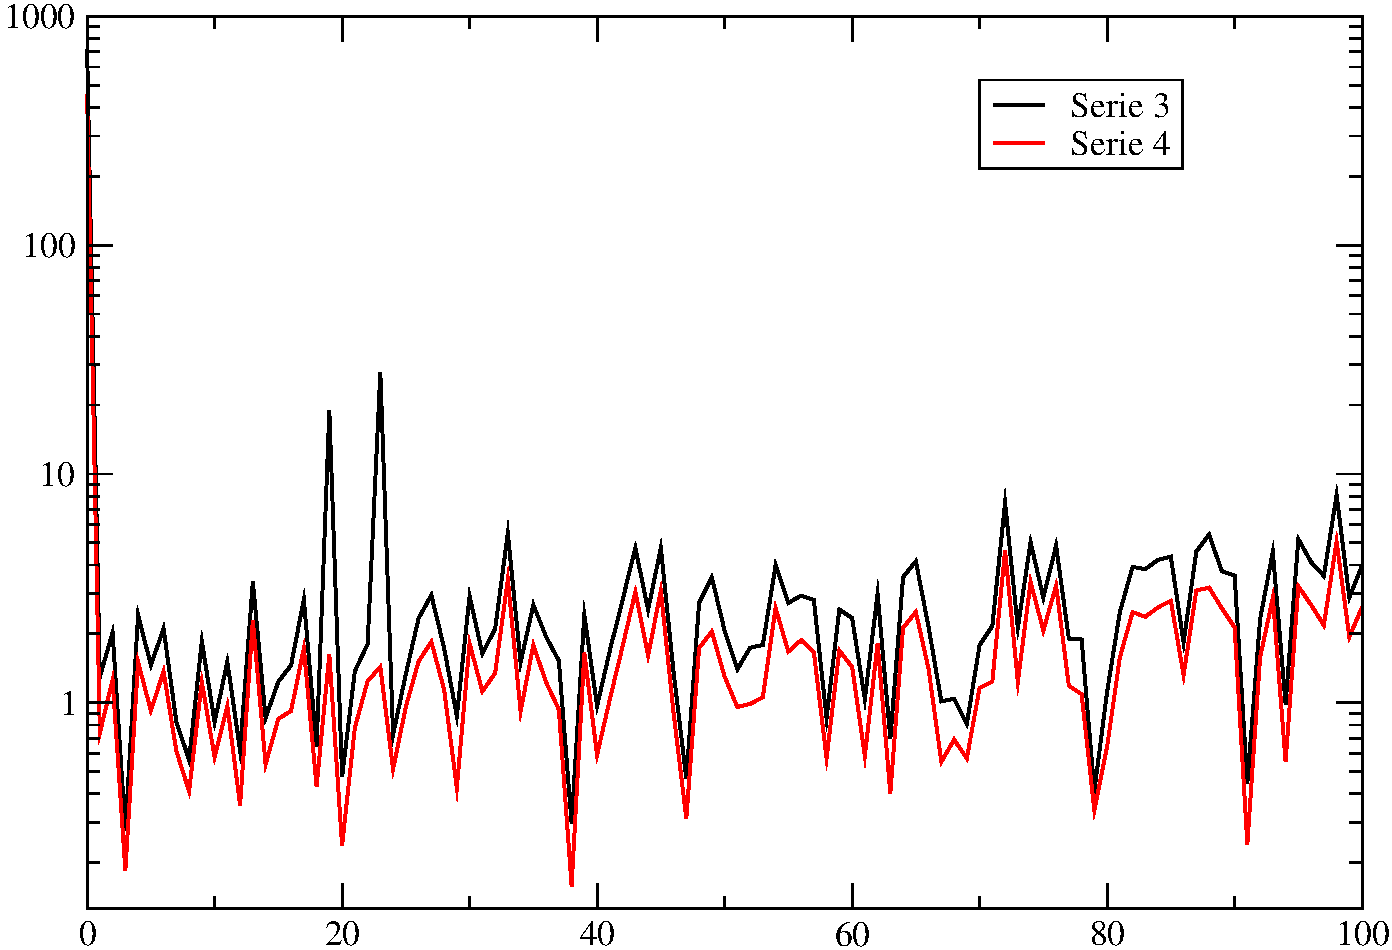
\includegraphics[width=0.447\textwidth]{saida4.pdf}
\caption{ Comparação do espectro de potência entre as séries 1 e 2 (esquerda) e séries 3 e 4 (direita).}
\label{pot}
\end{figure}




\subsection*{b)}
A frequência de Nyquist, dada por $f_{nyquist} = \frac{1}{2\Delta}$, é a frequência máxima que pode ser obtida por uma transformada de Fourier. Ela está relacionada ao intervalo $\Delta$ entre os pontos experimentais. Um lado positivo é que caso se saiba que um sinal possui um limitante superior de frequência este sinal pode ser reconstruido a partir de um número finito de pontos.

Em nosso caso, temos $\Delta = 3.26\times10^{-4}$ para as séries 1 e 2 e $\Delta = 2.44\times10^{-3}$ para as séries 3 e 4. Assim, $f_{nyquist} = 1.5 \times 10^{3} Hz$ para as séries 1 e 2 e $f_{nyquist} = 2.0 \times 10^{2}Hz$ para as séries 3 e 4.

\subsection*{c)}
Para que FFT possa ser utilizado N deve ser uma potência de 2. No nosso caso, $N = 1024 = 2^{10}$. Caso N não cumpra essa exigência a maneira mais fácil de contorna-la é adicionar zeros até que seja cumprida. O algoritmo da referência [2] não foi utilizado devido ao fato do programa enviar para subrotina um vetor de tamanho N e receber na subrotina um vetor de tamanho 1. Por não entender isto, foi utilizado o algoritmo da referência [3], cujo resultado pode ser visto no programa fft.f90. 

\begin{figure}[!htb]
\centering
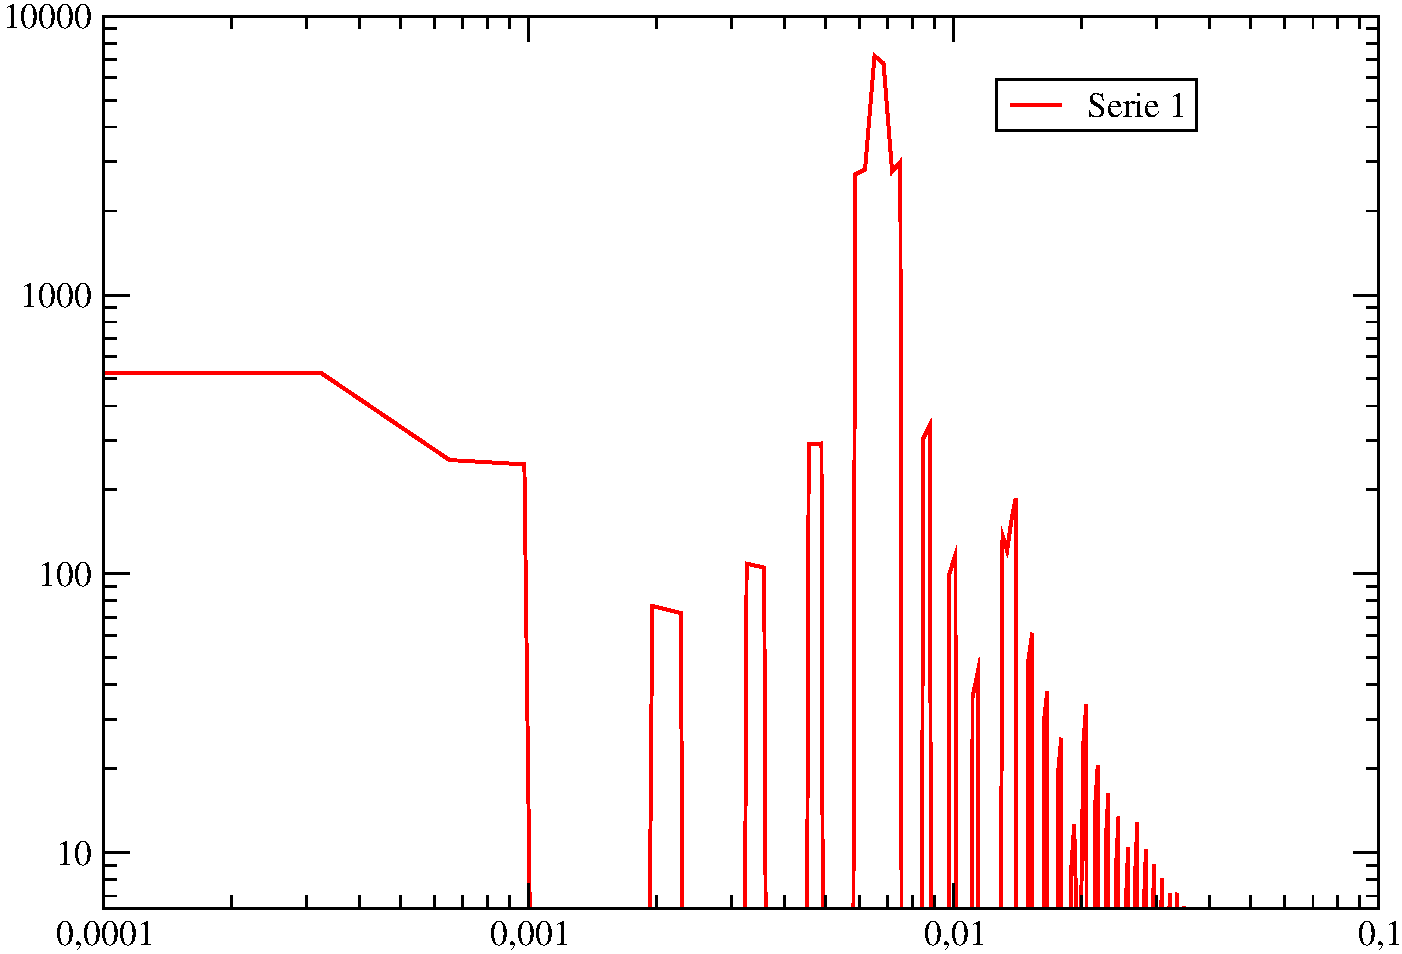
\includegraphics[width=0.447\textwidth]{fft.pdf}
\caption{ Comparação do espectro de potência entre a série 1 utilizando o algoritmo descrito em [3].}
\label{3c}
\end{figure}

O espectro obtido claramente não está de acordo com a Figura \ref{pot}. Como este espectro não parece fazer sentido algum erro deve ter sido feito na implementação do programa e as outras séries nem serão testadas.

\section*{Exercício 4}

Na Figura \ref{jk} foi plotado $J_k$ em função de $t_k$ para vermos como é o comportamento qualitativo da função. Como pode ser observado a função parece tender a zero quando t tende a zero e a derivada de $J_k$ claramente tende a zero quando $t\rightarrow \infty$.
\subsection*{a)}
\begin{figure}[!htb]
\centering
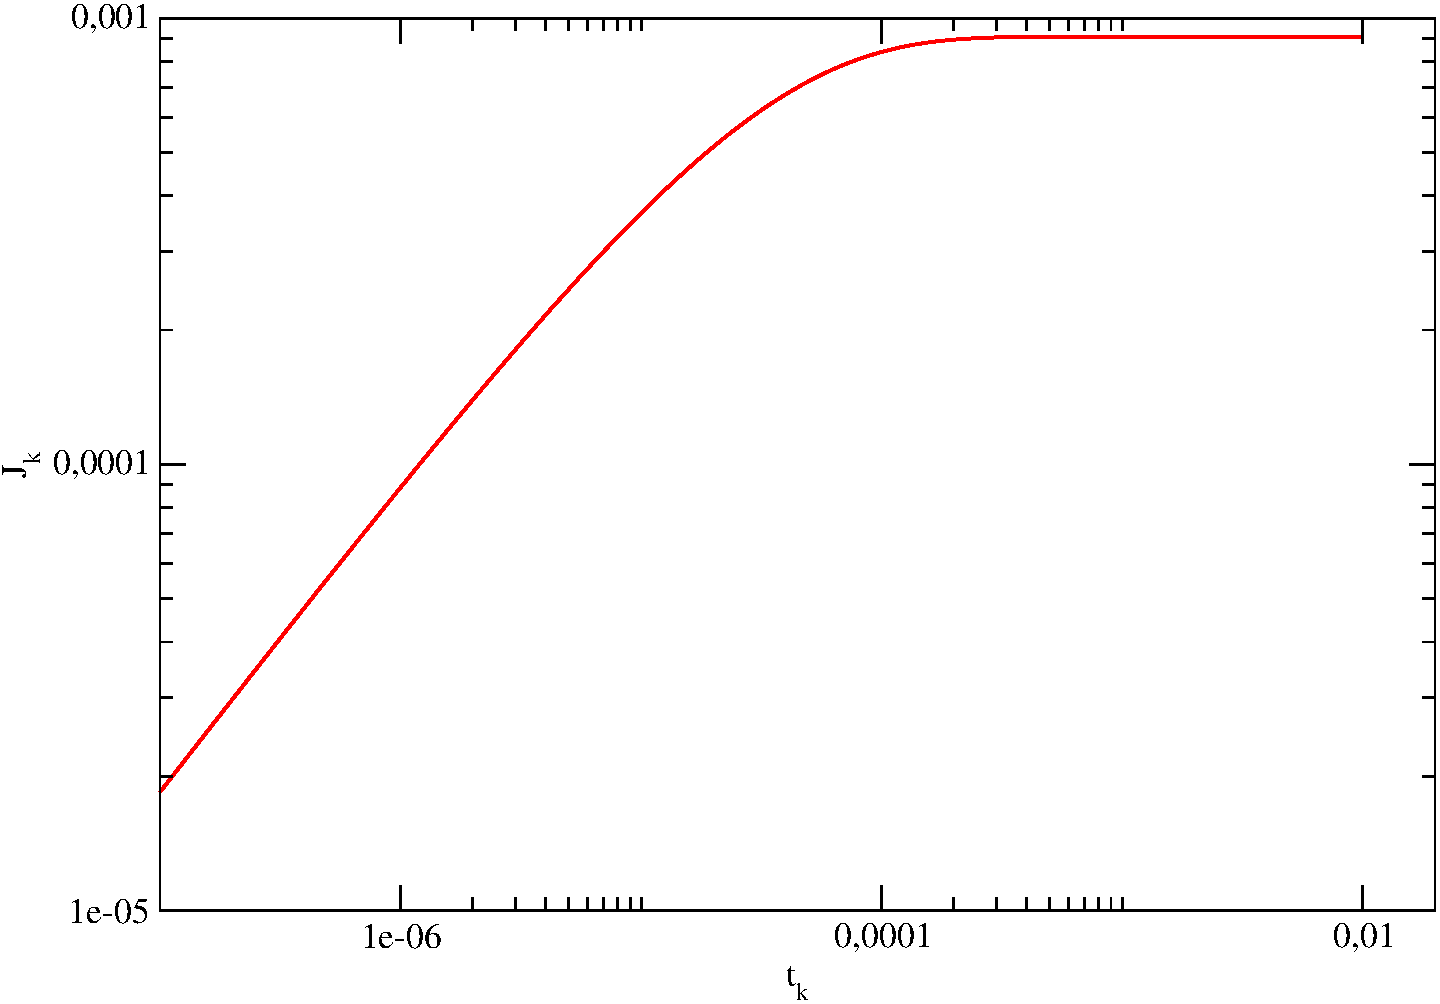
\includegraphics[width=0.447\textwidth]{jk.pdf}
\caption{ $J_k$ em função de $t_k$.}
\label{jk}
\end{figure}

Na Figura \ref{j} temos o comportamento das partes real e imaginária de J. As duas grandezas são negativas, portanto foi necessário multiplica-las por -1 para fazer o gráfico log-log.

\begin{figure}[!htb]
\centering
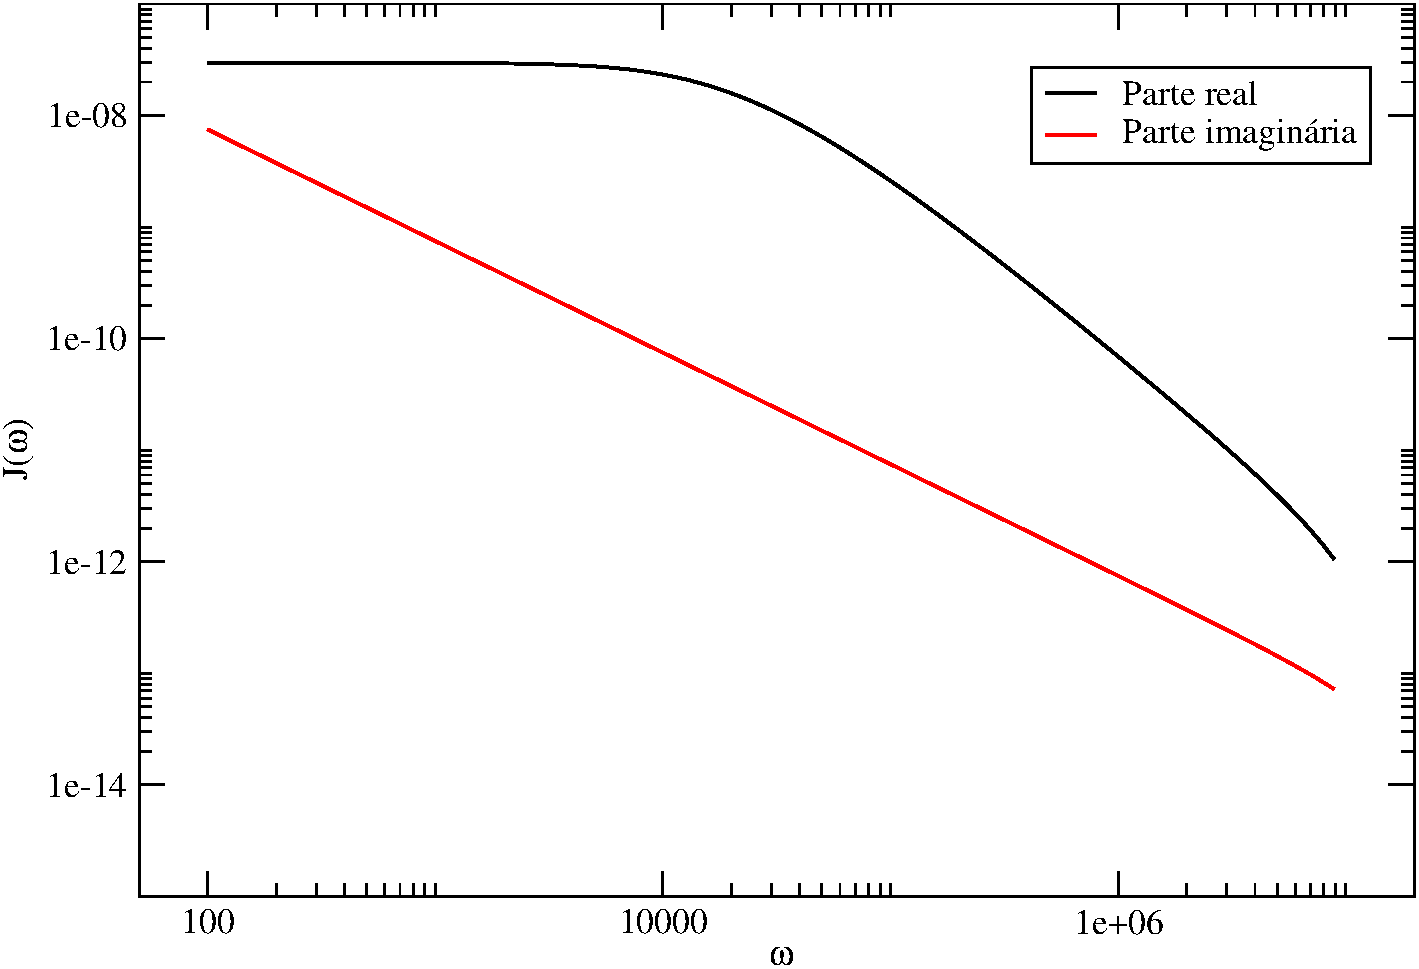
\includegraphics[width=0.447\textwidth]{J.pdf}
\caption{ Módulo das partes reais e imaginárias de $J$.}
\label{j}
\end{figure}


\subsection*{b)}
Na Figura \ref{g} estão respresentadas as partes real e imaginária da função G($\omega$).

\begin{figure}[!htb]
\centering
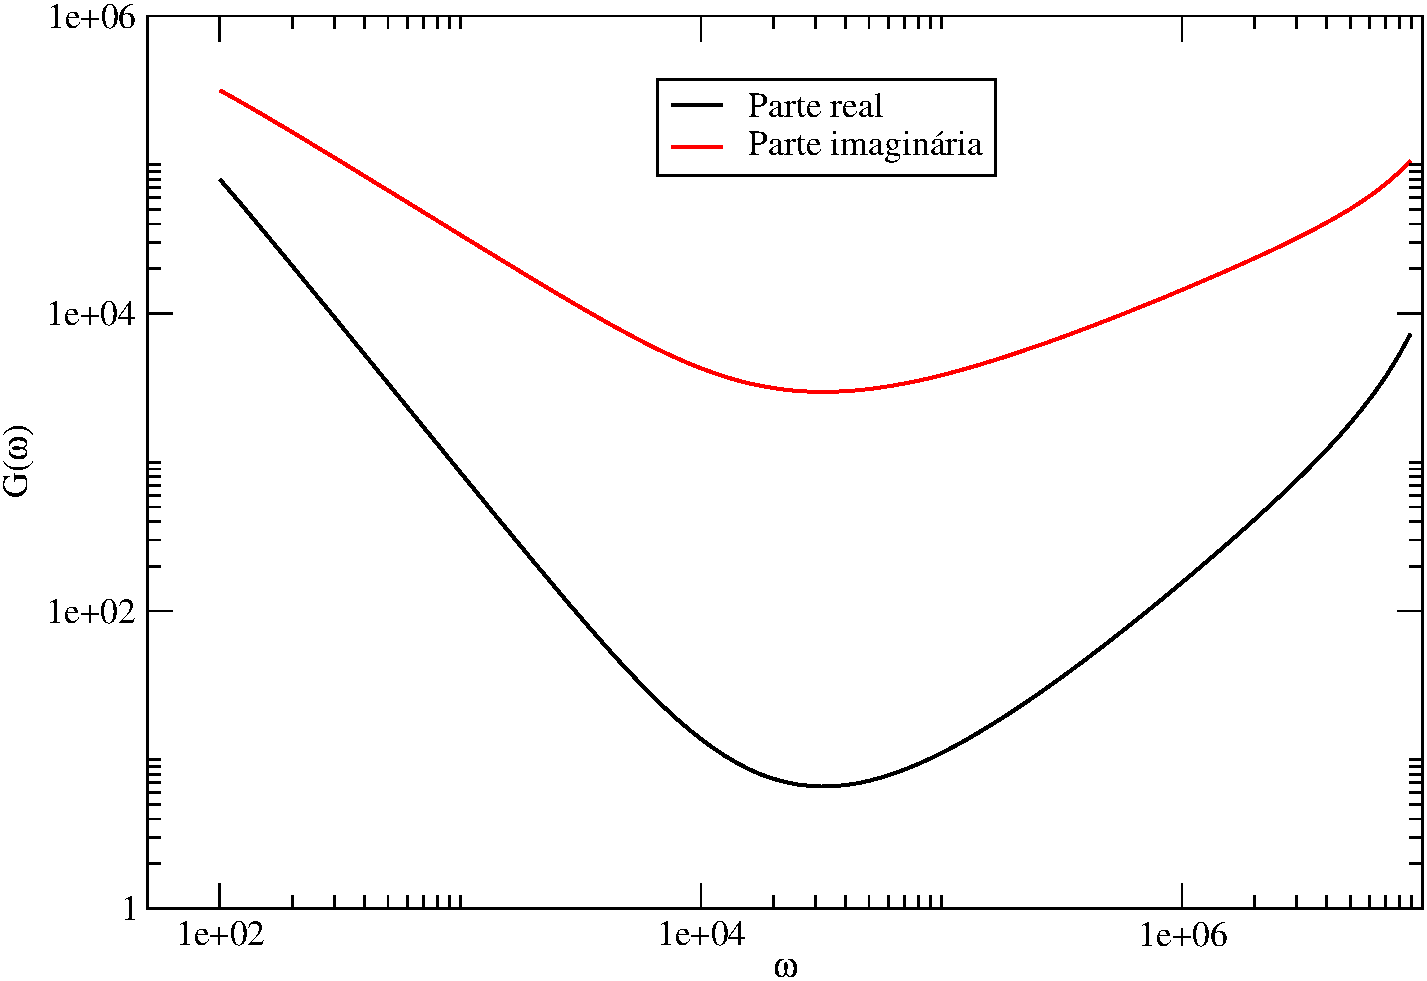
\includegraphics[width=0.447\textwidth]{g.pdf}
\caption{ Parte real e imaginária de G($\omega$).}
\label{g}
\end{figure}

\end{document}
